\documentclass[titlepage]{article}
\usepackage{listings}
\lstMakeShortInline{|}
\usepackage{courier}
%\usepackage{hyperref}
\usepackage[colorlinks,linkcolor=blue,citecolor=blue,urlcolor=blue,breaklinks=true]{hyperref}
\lstset{basicstyle=\ttfamily\small , breaklines}
%\usepackage[margin=2cm]{geometry}
\usepackage[left=3cm,top=3cm,bottom=3cm, right=3cm,includehead,includefoot,landscape]{geometry}
\usepackage{color}
\usepackage{fancyhdr,lastpage}
\pagestyle{fancy}
\rhead{Metrum Research Group, LLC \\ }
\lhead{
\includegraphics[scale=2]{logo.png}}
\cfoot{Page \thepage\ of \pageref{LastPage}}
\fancyhfoffset{.25in}
\renewcommand{\headrulewidth}{0.25pt}
\renewcommand{\footrulewidth}{0pt} 
\setlength{\headheight}{23pt}
\renewcommand{\labelitemiii}{$\circ$}
\usepackage{longtable}
\usepackage{amsmath}
\usepackage[T1]{fontenc}
\usepackage[scaled]{helvet}
\renewcommand*\familydefault{\sfdefault}
\usepackage{courier}
\usepackage{graphicx}
\usepackage{tocbibind}
\usepackage[parfill]{parskip}    % Activate to begin paragraphs with an empty line rather than an indent
\usepackage{upgreek}
\usepackage{textpos}
\usepackage{relsize}
\usepackage{upquote}
% Use \begin{landscape} and end{landscape} to rotate text %%%
\usepackage{pdflscape}
\usepackage{textcomp}
\usepackage{float}
\floatplacement{figure}{H}
\floatplacement{table}{H}
\usepackage[printonlyused,nohyperlinks]{acronym}
\def\bflabel#1{{\large#1\ \ \ \ }\hfill}
\usepackage{fixltx2e}
\setlength{\belowcaptionskip}{10pt}





\usepackage{Sweave}

 
\begin{document}
\vspace*{2cm}
\begin{center}
{\Large Modeling}\\
~\\
\today\\
~\\
Tim Bergsma\\
\end{center}
\newpage

\section{Purpose}
This script runs NONMEM models and diagnostics for sample phase1 data.
\section{Model Development}
\subsection{Set up for NONMEM run.}
\begin{Schunk}
\begin{Sinput}
> library(metrumrg)
\end{Sinput}
\begin{Soutput}
metrumrg 5.4 
enter "?metrumrg" for help
\end{Soutput}
\begin{Sinput}
> command <- '/opt/NONMEM/nm72/nmqual/autolog.pl'
> cat.cov='SEX'
> cont.cov=c('HEIGHT','WEIGHT','AGE')
> par.list=c('CL','Q','KA','V','V2','V3')
> eta.list=paste('ETA',1:10,sep='')
\end{Sinput}
\end{Schunk}
\subsection{Run NONMEM.}
\begin{Schunk}
\begin{Sinput}
> NONR72(
+      run=1001:1005,
+      command=command,
+      project='../nonmem',
+      grid=FALSE,
+      nice=TRUE,
+      checkrunno=FALSE,
+      cont.cov=cont.cov,
+      cat.cov=cat.cov,
+      par.list=par.list,
+      eta.list=eta.list,
+      plotfile='../nonmem/*/diagnostics.pdf',
+      streams='../nonmem/ctl',
+      checksum=FALSE
+ )
\end{Sinput}
\end{Schunk}
Covariance succeeded on model 1005.
We can make a quick run log using some simple tools. Table \ref{runlog}.
\begin{Schunk}
\begin{Sinput}
> log <- rlog(1001:1005,'../nonmem',tool='nm7')
> head(log)
\end{Sinput}
\begin{Soutput}
  tool  run parameter   moment            value
1  nm7 1001       ofv  minimum 2526.39867230031
2  nm7 1001    THETA1 estimate          11.7167
3  nm7 1001    THETA1     prse             8.67
4  nm7 1001    THETA1       se          1.01636
5  nm7 1001    THETA2 estimate          14.5657
6  nm7 1001    THETA2     prse             8.67
\end{Soutput}
\begin{Sinput}
> tail(log)
\end{Sinput}
\begin{Soutput}
    tool  run parameter   moment
245  nm7 1005  SIGMA2.2     prse
246  nm7 1005  SIGMA2.2       se
247  nm7 1005       cov   status
248  nm7 1005      prob     text
249  nm7 1005       min   status
250  nm7 1005      data filename
                                                  value
245                                                33.5
246                                           0.0676412
247                                                   0
248 1005 phase1 2 CMT like 1004 but diff. initial on V3
249                                                   0
250                       ../../data/derived/phase1.csv
\end{Soutput}
\begin{Sinput}
> sapply(log,class)
\end{Sinput}
\begin{Soutput}
       tool         run   parameter      moment       value 
"character"   "integer" "character" "character" "character" 
\end{Soutput}
\begin{Sinput}
> log$tool <- NULL
> unique(log$parameter)
\end{Sinput}
\begin{Soutput}
 [1] "ofv"      "THETA1"   "THETA2"   "THETA3"   "OMEGA1.1" "OMEGA2.1"
 [7] "OMEGA2.2" "OMEGA3.1" "OMEGA3.2" "OMEGA3.3" "SIGMA1.1" "SIGMA2.1"
[13] "SIGMA2.2" "cov"      "prob"     "min"      "data"     "THETA4"  
[19] "THETA5"   "OMEGA4.1" "OMEGA4.2" "OMEGA4.3" "OMEGA4.4" "OMEGA5.1"
[25] "OMEGA5.2" "OMEGA5.3" "OMEGA5.4" "OMEGA5.5" "THETA6"   "THETA7"  
\end{Soutput}
\begin{Sinput}
> log <- log[log$parameter %in% c('ofv','prob','cov','min'),]
> log
\end{Sinput}
\begin{Soutput}
     run parameter  moment
1   1001       ofv minimum
38  1001       cov  status
39  1001      prob    text
40  1001       min  status
42  1002       ofv minimum
112 1002       cov  status
113 1002      prob    text
114 1002       min  status
116 1003       ofv minimum
153 1003       cov  status
154 1003      prob    text
155 1003       min  status
157 1004       ofv minimum
194 1004       cov  status
195 1004      prob    text
196 1004       min  status
198 1005       ofv minimum
247 1005       cov  status
248 1005      prob    text
249 1005       min  status
                                                          value
1                                              2526.39867230031
38                                                            0
39                                             1001 phase1 1CMT
40                                                            0
42                                             2525.96526753388
112                                                           1
113                                           1002 phase1 2 CMT
114                                                           1
116                                            2569.89393760215
153                                                           1
154 1003 phase1 2 CMT like 1002 but no eta on Q/v3 and no + err
155                                                           0
157                                            2570.45022637547
194                                                           0
195               1004 phase1 2 CMT like 1003 but better bounds
196                                                           0
198                                            2405.91625845151
247                                                           0
248         1005 phase1 2 CMT like 1004 but diff. initial on V3
249                                                           0
\end{Soutput}
\begin{Sinput}
> with(log, constant(moment,within=parameter))#i.e., moment is non-informative here.
\end{Sinput}
\begin{Soutput}
[1] TRUE
\end{Soutput}
\begin{Sinput}
> log <- data.frame(cast(log,run~parameter))
> log <- shuffle(log,'prob','run')
> log$ofv <- signif(as.numeric(as.character(log$ofv,6)))
\end{Sinput}
\end{Schunk}
\begin{table}[!htpb]
 \caption[Run Log]{Run Log \label{runlog}}
 \begin{center}
  \begin{tabular}{rlllr}
    \hline \hline
   run & prob & cov & min & ofv \\ \hline
   \verb#1001# & 1001 phase1 1CMT                                            & 0 & 0 & \verb#2526.40# \\
   \verb#1002# & 1002 phase1 2 CMT                                           & 1 & 1 & \verb#2525.97# \\
   \verb#1003# & 1003 phase1 2 CMT like 1002 but no eta on Q/v3 and no + err & 1 & 0 & \verb#2569.89# \\
   \verb#1004# & 1004 phase1 2 CMT like 1003 but better bounds               & 0 & 0 & \verb#2570.45# \\
   \verb#1005# & 1005 phase1 2 CMT like 1004 but diff. initial on V3         & 0 & 0 & \verb#2405.92# \\ \hline
  \end{tabular}
 \end{center}
\end{table}\section{Predictive Check}
\subsection{Create a simulation control stream.}
Convert control stream to R object.
\begin{Schunk}
\begin{Sinput}
> ctl <- read.nmctl('../nonmem/ctl/1005.ctl')
\end{Sinput}
\end{Schunk}
Strip comments and view.
\begin{Schunk}
\begin{Sinput}
> ctl[] <- lapply(ctl,function(rec)sub(' *;.*','',rec))
> ctl
\end{Sinput}
\begin{Soutput}
 [1] "$PROB 1005 phase1 2 CMT like 1004 but diff. initial on V3"                                   
 [2] "$INPUT C ID TIME SEQ=DROP EVID AMT DV SUBJ HOUR TAFD TAD LDOS MDV HEIGHT WT SEX AGE DOSE FED"
 [3] "$DATA ../../data/derived/phase1.csv IGNORE=C"                                                
 [4] "$SUBROUTINE ADVAN4 TRANS4"                                                                   
 [5] "$PK"                                                                                         
 [6] " CL=THETA(1)*EXP(ETA(1)) * THETA(6)**SEX * (WT/70)**THETA(7)"                                
 [7] " V2 =THETA(2)*EXP(ETA(2))"                                                                   
 [8] " KA=THETA(3)*EXP(ETA(3))"                                                                    
 [9] " Q  =THETA(4)"                                                                               
[10] " V3=THETA(5)"                                                                                
[11] " S2=V2"                                                                                      
[12] " "                                                                                           
[13] "$ERROR"                                                                                      
[14] " Y=F*(1+ERR(1)) + ERR(2)"                                                                    
[15] " IPRE=F"                                                                                     
[16] ""                                                                                            
[17] "$THETA"                                                                                      
[18] "(0,10,50)"                                                                                   
[19] "(0,10,100)"                                                                                  
[20] "(0,0.2, 5)"                                                                                  
[21] "(0,10,50)"                                                                                   
[22] "(0,100,1000)"                                                                                
[23] "(0,1,2)"                                                                                     
[24] "(0,0.75,3)"                                                                                  
[25] ""                                                                                            
[26] "$OMEGA BLOCK(3)"                                                                             
[27] ".1"                                                                                          
[28] ".01 .1"                                                                                      
[29] ".01 .01 .1"                                                                                  
[30] ""                                                                                            
[31] ""                                                                                            
[32] ""                                                                                            
[33] ""                                                                                            
[34] ""                                                                                            
[35] ""                                                                                            
[36] ""                                                                                            
[37] ""                                                                                            
[38] "$SIGMA 0.1 0.1"                                                                              
[39] ""                                                                                            
[40] ""                                                                                            
[41] ""                                                                                            
[42] ""                                                                                            
[43] "$ESTIMATION MAXEVAL=9999 PRINT=5 NOABORT METHOD=1 INTER MSFO=./1005.msf"                     
[44] "$COV PRINT=E"                                                                                
[45] "$TABLE NOPRINT FILE=./1005.tab ONEHEADER ID AMT TIME EVID PRED IPRE CWRES"                   
[46] "$TABLE NOPRINT FILE=./1005par.tab ONEHEADER ID TIME CL Q V2 V3 KA ETA1 ETA2 ETA3"            
[47] ""                                                                                            
[48] ""                                                                                            
[49] ""                                                                                            
[50] ""                                                                                            
[51] ""                                                                                            
[52] ""                                                                                            
[53] ""                                                                                            
[54] ""                                                                                            
[55] ""                                                                                            
[56] ""                                                                                            
[57] ""                                                                                            
[58] ""                                                                                            
[59] ""                                                                                            
[60] ""                                                                                            
[61] ""                                                                                            
[62] ""                                                                                            
[63] ""                                                                                            
\end{Soutput}
\end{Schunk}
Fix records of interest.
\begin{Schunk}
\begin{Sinput}
> ctl$prob
\end{Sinput}
\begin{Soutput}
[1] "1005 phase1 2 CMT like 1004 but diff. initial on V3"
\end{Soutput}
\begin{Sinput}
> ctl$prob <- sub('1005','1105',ctl$prob)
> names(ctl)
\end{Sinput}
\begin{Soutput}
 [1] "prob"       "input"      "data"       "subroutine" "pk"        
 [6] "error"      "theta"      "omega"      "sigma"      "estimation"
[11] "cov"        "table"      "table"     
\end{Soutput}
\begin{Sinput}
> names(ctl)[names(ctl)=='theta'] <- 'msfi'
> ctl$msfi <- '=../1005/1005.msf'
> ctl$omega <- NULL
> ctl$sigma <- NULL
> names(ctl)[names(ctl)=='estimation'] <- 'simulation'
> ctl$simulation <- 'ONLYSIM (1968) SUBPROBLEMS=500'
> ctl$cov <- NULL
> ctl$table <- NULL
> ctl$table <- NULL
> ctl$table <- 'DV NOHEADER NOPRINT FILE=./1105.tab FORWARD NOAPPEND'
> write.nmctl(ctl,'../nonmem/ctl/1105.ctl')
\end{Sinput}
\end{Schunk}
\subsection{Run the simulation.}
This run makes the predictions (simulations).
\begin{Schunk}
\begin{Sinput}
> NONR72(
+      run=1105,
+      command=command,
+      project='../nonmem',
+      grid=FALSE,
+      nice=TRUE,
+      diag=FALSE,
+      streams='../nonmem/ctl',
+      checksum=FALSE
+ )
\end{Sinput}
\end{Schunk}
\subsection{Recover and format the original dataset.}
Now we fetch the results and integrate them with the other data.
\begin{Schunk}
\begin{Sinput}
> phase1 <- read.csv('../data/derived/phase1.csv',na.strings='.')
> head(phase1)
\end{Sinput}
\begin{Soutput}
     C ID TIME SEQ EVID  AMT    DV SUBJ HOUR TAFD  TAD LDOS MDV HEIGHT WEIGHT
1    C  1 0.00   0    0   NA 0.000    1 0.00 0.00   NA   NA   0    174   74.2
2 <NA>  1 0.00   1    1 1000    NA    1 0.00 0.00 0.00 1000   1    174   74.2
3 <NA>  1 0.25   0    0   NA 0.363    1 0.25 0.25 0.25 1000   0    174   74.2
4 <NA>  1 0.50   0    0   NA 0.914    1 0.50 0.50 0.50 1000   0    174   74.2
5 <NA>  1 1.00   0    0   NA 1.120    1 1.00 1.00 1.00 1000   0    174   74.2
6 <NA>  1 2.00   0    0   NA 2.280    1 2.00 2.00 2.00 1000   0    174   74.2
  SEX  AGE DOSE FED SMK DS CRCN predose zerodv
1   0 29.1 1000   1   0  0 83.5       1      0
2   0 29.1 1000   1   0  0 83.5       0      0
3   0 29.1 1000   1   0  0 83.5       0      0
4   0 29.1 1000   1   0  0 83.5       0      0
5   0 29.1 1000   1   0  0 83.5       0      0
6   0 29.1 1000   1   0  0 83.5       0      0
\end{Soutput}
\begin{Sinput}
> phase1 <- phase1[is.na(phase1$C),c('SUBJ','TIME','DV')]
> records <- nrow(phase1)
> records
\end{Sinput}
\begin{Soutput}
[1] 550
\end{Soutput}
\begin{Sinput}
> phase1 <- phase1[rep(1:records,500),]
> nrow(phase1)
\end{Sinput}
\begin{Soutput}
[1] 275000
\end{Soutput}
\begin{Sinput}
> phase1$SIM <- rep(1:500,each=records)
> #head(phase1,300)
> with(phase1,DV[SIM==1 & SUBJ==12])
\end{Sinput}
\begin{Soutput}
 [1]     NA  2.260  2.830  8.730 19.300 15.200 16.200  8.830 12.900 12.700
[11]  7.140  5.740  1.980  0.791
\end{Soutput}
\begin{Sinput}
> with(phase1,DV[SIM==2 & SUBJ==12])
\end{Sinput}
\begin{Soutput}
 [1]     NA  2.260  2.830  8.730 19.300 15.200 16.200  8.830 12.900 12.700
[11]  7.140  5.740  1.980  0.791
\end{Soutput}
\end{Schunk}
\subsection{Recover and format the simulation results.}
\begin{Schunk}
\begin{Sinput}
> pred <- scan('../nonmem/1105/1105.tab')
> nrow(phase1)
\end{Sinput}
\begin{Soutput}
[1] 275000
\end{Soutput}
\begin{Sinput}
> length(pred)
\end{Sinput}
\begin{Soutput}
[1] 275000
\end{Soutput}
\end{Schunk}
\subsection{Combine the original data and the simulation data.}
\begin{Schunk}
\begin{Sinput}
> phase1$PRED <- pred
> head(phase1)
\end{Sinput}
\begin{Soutput}
  SUBJ TIME    DV SIM    PRED
2    1 0.00    NA   1 0.00000
3    1 0.25 0.363   1 0.72542
4    1 0.50 0.914   1 1.38320
5    1 1.00 1.120   1 2.06720
6    1 2.00 2.280   1 3.48570
7    1 3.00 1.630   1 5.44600
\end{Soutput}
\begin{Sinput}
> phase1 <- phase1[!is.na(phase1$DV),]
> head(phase1)
\end{Sinput}
\begin{Soutput}
  SUBJ TIME    DV SIM    PRED
3    1 0.25 0.363   1 0.72542
4    1 0.50 0.914   1 1.38320
5    1 1.00 1.120   1 2.06720
6    1 2.00 2.280   1 3.48570
7    1 3.00 1.630   1 5.44600
8    1 4.00 2.040   1 2.99140
\end{Soutput}
\end{Schunk}
\subsection{Plot predictive checks.}
\subsubsection{Aggregate data within subject.}
Since subjects may contribute differing numbers of observations, it may
be useful to look at predictions from a subject-centric perspective.
Therefore, we wish to calculate summary statistics for each subject, 
(observed and predicted) and then make obspred comparisons therewith.
\begin{Schunk}
\begin{Sinput}
> head(phase1)
\end{Sinput}
\begin{Soutput}
  SUBJ TIME    DV SIM    PRED
3    1 0.25 0.363   1 0.72542
4    1 0.50 0.914   1 1.38320
5    1 1.00 1.120   1 2.06720
6    1 2.00 2.280   1 3.48570
7    1 3.00 1.630   1 5.44600
8    1 4.00 2.040   1 2.99140
\end{Soutput}
\begin{Sinput}
> subject <- melt(phase1,measure.var=c('DV','PRED'))
> head(subject)
\end{Sinput}
\begin{Soutput}
  SUBJ TIME SIM variable value
1    1 0.25   1       DV 0.363
2    1 0.50   1       DV 0.914
3    1 1.00   1       DV 1.120
4    1 2.00   1       DV 2.280
5    1 3.00   1       DV 1.630
6    1 4.00   1       DV 2.040
\end{Soutput}
\end{Schunk}
We are going to aggregate each subject's DV and PRED values using cast().
cast() likes an aggregation function that returns a list.
We write one that grabs min med max for each subject, sim, and variable.
\begin{Schunk}
\begin{Sinput}
> metrics <- function(x)list(min=min(x), med=median(x), max=max(x))
\end{Sinput}
\end{Schunk}
Now we cast, ignoring time.
\begin{Schunk}
\begin{Sinput}
> subject <- data.frame(cast(subject, SUBJ + SIM + variable ~ .,fun=metrics))
> head(subject)
\end{Sinput}
\begin{Soutput}
  SUBJ SIM variable       min    med     max
1    1   1       DV  0.363000 1.6100  3.0900
2    1   1     PRED  0.725420 3.4795  5.4460
3    1   2       DV  0.363000 1.6100  3.0900
4    1   2     PRED -0.085238 2.2941  4.6468
5    1   3       DV  0.363000 1.6100  3.0900
6    1   3     PRED -0.022407 4.8896 12.3770
\end{Soutput}
\end{Schunk}
Note that regardless of SIM, DV (observed) is constant.

Now we melt the metrics.
\begin{Schunk}
\begin{Sinput}
> metr <- melt(subject,measure.var=c('min','med','max'),variable_name='metric')
> head(metr)
\end{Sinput}
\begin{Soutput}
  SUBJ SIM variable metric     value
1    1   1       DV    min  0.363000
2    1   1     PRED    min  0.725420
3    1   2       DV    min  0.363000
4    1   2     PRED    min -0.085238
5    1   3       DV    min  0.363000
6    1   3     PRED    min -0.022407
\end{Soutput}
\begin{Sinput}
> metr$value <- reapply(
+ 	metr$value,
+ 	INDEX=metr[,c('SIM','variable','metric')],
+ 	FUN=sort,
+ 	na.last=FALSE
+ )
> metr <- data.frame(cast(metr))
> head(metr)
\end{Sinput}
\begin{Soutput}
  SUBJ SIM metric    DV     PRED
1    1   1    min 0.139 -0.61537
2    1   1    med 1.025  1.25865
3    1   1    max 2.530  2.17620
4    1   2    min 0.139 -0.35196
5    1   2    med 1.025  1.20926
6    1   2    max 2.530  2.42390
\end{Soutput}
\begin{Sinput}
> nrow(metr)
\end{Sinput}
\begin{Soutput}
[1] 60000
\end{Soutput}
\begin{Sinput}
> metr <- metr[!is.na(metr$DV),]#maybe no NA
> nrow(metr)
\end{Sinput}
\begin{Soutput}
[1] 60000
\end{Soutput}
\end{Schunk}
We plot using lattice.
\begin{Schunk}
\begin{Sinput}
> print(
+ 	xyplot(
+ 		PRED~DV|metric,
+ 		metr,
+ 		groups=SIM,
+ 		scales=list(relation='free'),
+ 		type='l',
+ 		panel=function(...){
+ 			panel.superpose(...)
+ 			panel.abline(0,1,col='white',lwd=2)
+ 		}
+ 	)
+ )
\end{Sinput}
\end{Schunk}
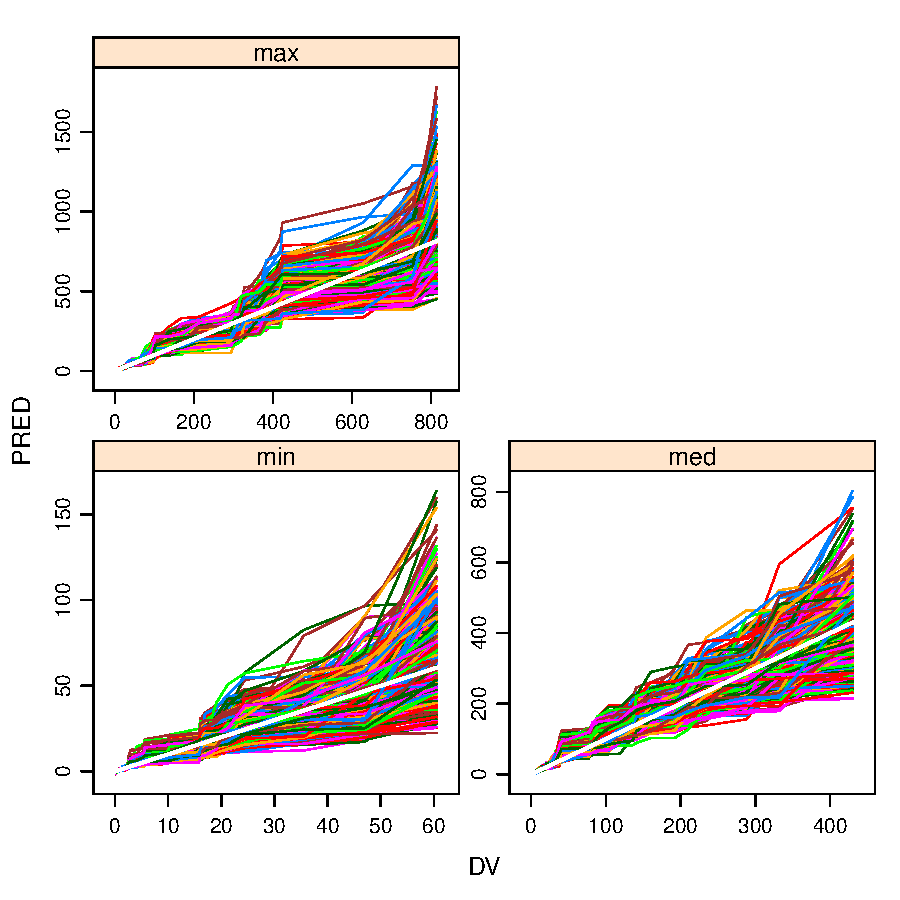
\includegraphics{model-qq}

For detail, we show one endpoint, tossing the outer 5 percent of values, and 
indicating quartiles.
\begin{Schunk}
\begin{Sinput}
> med <- metr[metr$metric=='med',]
> med$metric <- NULL
> head(med)
\end{Sinput}
\begin{Soutput}
   SUBJ SIM    DV    PRED
2     1   1 1.025 1.25865
5     1   2 1.025 1.20926
8     1   3 1.025 1.57990
11    1   4 1.025 0.88489
14    1   5 1.025 1.65875
17    1   6 1.025 0.95005
\end{Soutput}
\begin{Sinput}
> trim <- inner(med, id.var=c('SIM'),measure.var=c('PRED','DV'))
> head(trim)
\end{Sinput}
\begin{Soutput}
  SIM DV PRED
1   1 NA   NA
2   2 NA   NA
3   3 NA   NA
4   4 NA   NA
5   5 NA   NA
6   6 NA   NA
\end{Soutput}
\begin{Sinput}
> nrow(trim)
\end{Sinput}
\begin{Soutput}
[1] 20000
\end{Soutput}
\begin{Sinput}
> trim <- trim[!is.na(trim$DV),]
> nrow(trim)
\end{Sinput}
\begin{Soutput}
[1] 19000
\end{Soutput}
\begin{Sinput}
> head(trim)
\end{Sinput}
\begin{Soutput}
    SIM   DV    PRED
501   1 1.13 2.05880
502   2 1.13 2.00535
503   3 1.13 1.65480
504   4 1.13 1.06910
505   5 1.13 2.05960
506   6 1.13 0.98589
\end{Soutput}
\begin{Sinput}
> print(
+ 	xyplot(
+ 		PRED~DV,
+ 		trim,
+ 		groups=SIM,
+ 		type='l',
+ 		panel=function(x,y,...){
+ 			panel.xyplot(x=x,y=y,...)
+ 			panel.abline(0,1,col='white',lwd=2)
+ 			panel.abline(
+ 				v=quantile(x,probs=c(0.25,0.5,0.75)),
+ 				col='grey',
+ 				lty=2
+ 			)
+ 		}
+ 	)
+ )
\end{Sinput}
\end{Schunk}
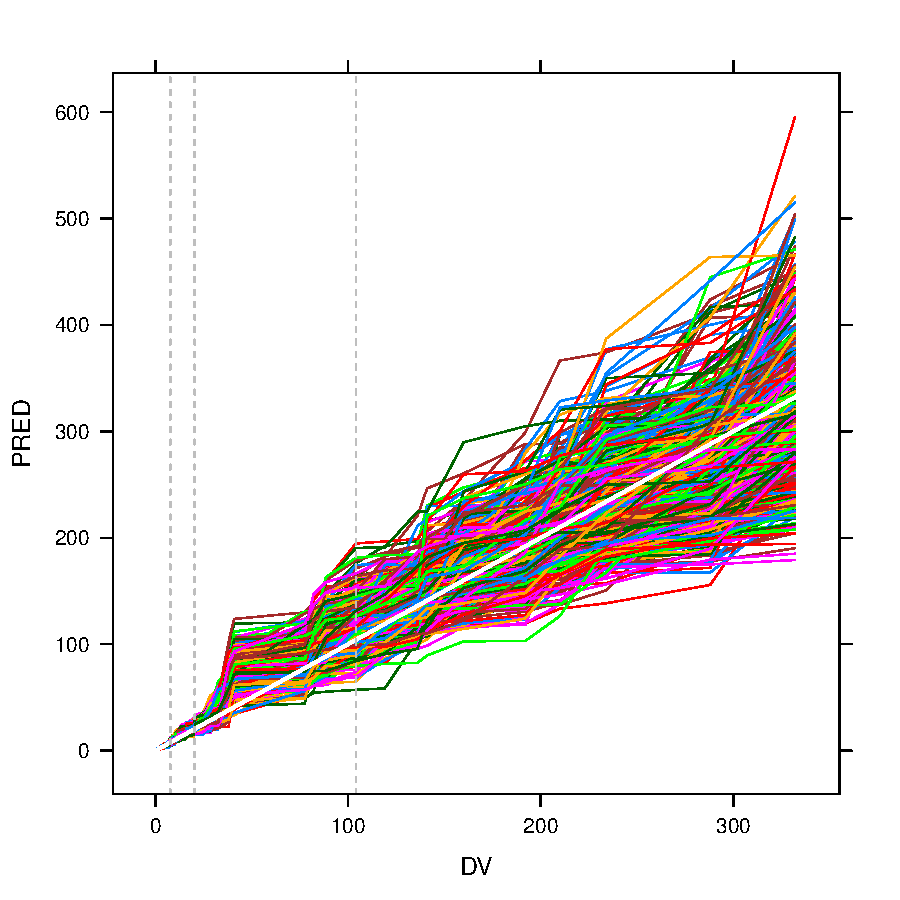
\includegraphics{model-qqdetail}

We also show densityplots of predictions at those quartiles.
\begin{Schunk}
\begin{Sinput}
> head(trim)
\end{Sinput}
\begin{Soutput}
    SIM   DV    PRED
501   1 1.13 2.05880
502   2 1.13 2.00535
503   3 1.13 1.65480
504   4 1.13 1.06910
505   5 1.13 2.05960
506   6 1.13 0.98589
\end{Soutput}
\begin{Sinput}
> quantile(trim$DV)
\end{Sinput}
\begin{Soutput}
    0%    25%    50%    75%   100% 
  1.13   7.69  20.25 104.00 332.00 
\end{Soutput}
\begin{Sinput}
> molt <- melt(trim, id.var='SIM')
> head(molt)
\end{Sinput}
\begin{Soutput}
  SIM variable value
1   1       DV  1.13
2   2       DV  1.13
3   3       DV  1.13
4   4       DV  1.13
5   5       DV  1.13
6   6       DV  1.13
\end{Soutput}
\begin{Sinput}
> quart <- data.frame(cast(molt,SIM+variable~.,fun=quantile,probs=c(0.25,0.5,0.75)))
> head(quart)
\end{Sinput}
\begin{Soutput}
  SIM variable     X25.     X50.      X75.
1   1       DV  7.95000 20.25000 100.10000
2   1     PRED 11.92825 22.16750 103.96500
3   2       DV  7.95000 20.25000 100.10000
4   2     PRED  7.23495 20.27050 105.20875
5   3       DV  7.95000 20.25000 100.10000
6   3     PRED  7.82690 14.50425  98.27575
\end{Soutput}
\begin{Sinput}
> molt <- melt(quart,id.var='variable',measure.var=c('X25.','X50.','X75.'),variable_name='quartile')
> head(molt)
\end{Sinput}
\begin{Soutput}
  variable quartile    value
1       DV     X25.  7.95000
2     PRED     X25. 11.92825
3       DV     X25.  7.95000
4     PRED     X25.  7.23495
5       DV     X25.  7.95000
6     PRED     X25.  7.82690
\end{Soutput}
\begin{Sinput}
> levels(molt$quartile)
\end{Sinput}
\begin{Soutput}
[1] "X25." "X50." "X75."
\end{Soutput}
\begin{Sinput}
> levels(molt$quartile) <- c('first quartile','second quartile','third quartile')
> head(molt)
\end{Sinput}
\begin{Soutput}
  variable       quartile    value
1       DV first quartile  7.95000
2     PRED first quartile 11.92825
3       DV first quartile  7.95000
4     PRED first quartile  7.23495
5       DV first quartile  7.95000
6     PRED first quartile  7.82690
\end{Soutput}
\begin{Sinput}
> levels(molt$variable)
\end{Sinput}
\begin{Soutput}
[1] "DV"   "PRED"
\end{Soutput}
\begin{Sinput}
> molt$variable <- factor(molt$variable,levels=c('PRED','DV'))
> print(
+ 	densityplot(
+ 		~value|quartile,
+ 		molt,
+ 		groups=variable,
+ 		layout=c(3,1),
+ 		scales=list(relation='free'),
+ 		aspect=1,
+ 		panel=panel.superpose,
+ 		panel.groups=function(x,...,group.number){
+ 			if(group.number==1)panel.densityplot(x,...)
+ 			if(group.number==2)panel.abline(v=unique(x),...)
+ 		},
+ 		auto.key=TRUE
+ 	)
+ )
\end{Sinput}
\end{Schunk}
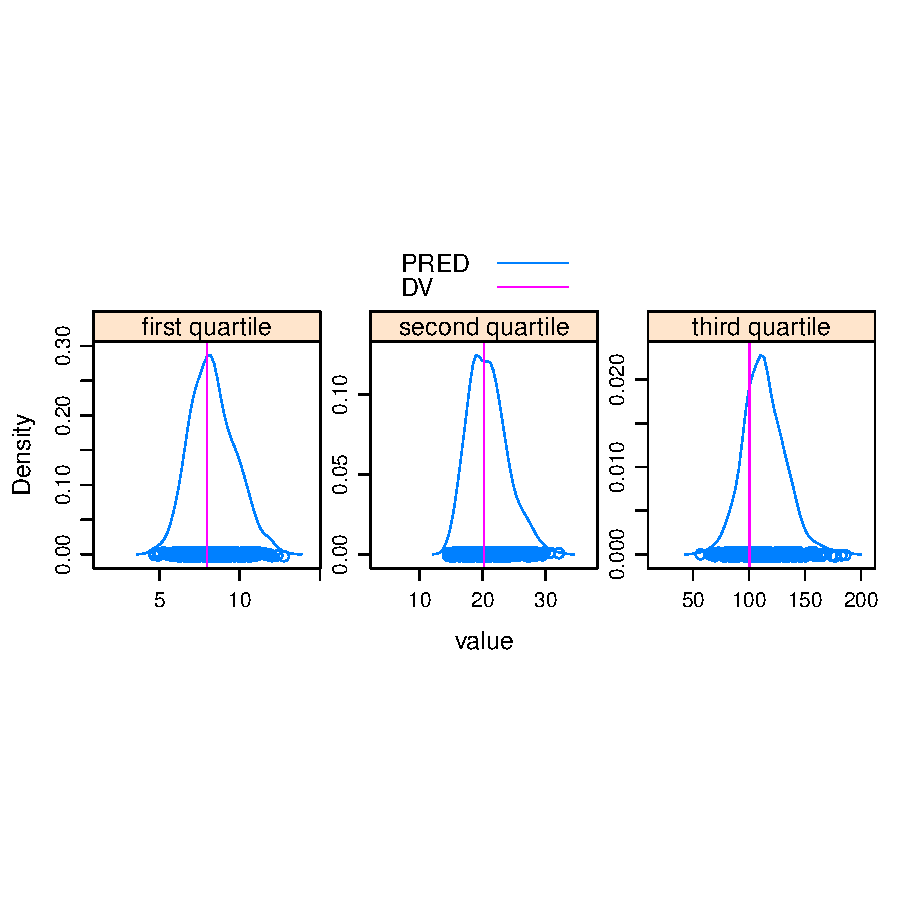
\includegraphics{model-qqdensity}
\section{Bootstrap Estimates of Parameter Uncertainty}
\subsection{Create directories.}
\begin{Schunk}
\begin{Sinput}
> getwd()
\end{Sinput}
\begin{Soutput}
[1] "/data/metsvn/wiki/inst/sample/script"
\end{Soutput}
\begin{Sinput}
> dir.create('../nonmem/1005.boot')
> dir.create('../nonmem/1005.boot/data')
> dir.create('../nonmem/1005.boot/ctl')
\end{Sinput}
\end{Schunk}
\subsection{Create replicate control streams.}
\begin{Schunk}
\begin{Sinput}
> t <- metaSub(
+      clear(readLines('../nonmem/ctl/1005.ctl'),';.+',fixed=FALSE),
+      names=1:300,
+      pattern=c(
+          '1005',
+          '../../data/derived/phase1.csv',
+          '$COV',
+          '$TABLE'
+      ),
+      replacement=c(
+          '*',
+          '../data/*.csv',
+          ';$COV',
+          ';$TABLE'
+     ),
+     fixed=TRUE,
+     out='../nonmem/1005.boot/ctl',
+     suffix='.ctl'
+  )
\end{Sinput}
\end{Schunk}
\subsection{Create replicate data sets by resampling original.}
\begin{Schunk}
\begin{Sinput}
>  bootset <- read.csv('../data/derived/phase1.csv')
>  r <- resample(
+  	bootset,
+  	names=1:300,
+  	key='ID',
+  	rekey=TRUE,
+  	out='../nonmem/1005.boot/data',
+  	stratify='SEX'
+  )
\end{Sinput}
\end{Schunk}
\subsection{Run bootstrap models.}
\begin{Schunk}
\begin{Sinput}
> NONR72(
+      run=1:300,
+      command=command,
+      project='../nonmem/1005.boot/',
+      boot=TRUE,
+      nice=TRUE,
+      grid=TRUE,
+      #concurrent=TRUE,
+      streams='../nonmem/1005.boot/ctl',
+      checksum=FALSE
+ )
\end{Sinput}
\begin{Soutput}
Installing SIGCHLD signal handler...Done.
\end{Soutput}
\begin{Sinput}
> nms <- paste('../nonmem/1005.boot/',1:300,'.boot/',1:300,'.log.xml',sep='')
> while(!(all(file.exists(nms))))Sys.sleep(10)
> boot <- rlog(
+ 	run=1:300,
+ 	project='../nonmem/1005.boot',
+ 	boot=TRUE,
+ 	append=FALSE,
+ 	tool='nm7'
+ )
> write.csv(boot, '../nonmem/1005.boot/log.csv')  
\end{Sinput}
\end{Schunk}
\end{document}
